% =====================================================================
% Mid-submission slides -- Team Ugh  (revision 2)
%
% HOW TO USE WITH YOUR OVERLEAF TEMPLATE (Universite Laval - Olico2):
%   1. Keep the template's own preamble (\documentclass, theme, colours, logos).
%   2. Copy the block marked "PACKAGES" into the template's preamble
%      (skip any package the template already loads).
%   3. Copy everything between \begin{document} and \end{document}.
%   4. Upload the figures/ folder (rq1_forest.pdf, scope_slope.pdf,
%      rq2_decomposition.pdf, probability_pairs.pdf).
% The "STANDALONE TEST" preamble only lets this file compile on its own.
% Figures are generated by scripts/make_slide_figures.py.
% =====================================================================

% ---------------- STANDALONE TEST (replace with template preamble) ----------
\documentclass[aspectratio=169,11pt]{beamer}
\usetheme{default}
\usecolortheme{seahorse}
\setbeamertemplate{navigation symbols}{}
\setbeamertemplate{footline}[frame number]
% ---------------------------------------------------------------------------

% ---------------- PACKAGES (copy into the template preamble) ----------------
\usepackage[T1]{fontenc}
\usepackage[utf8]{inputenc}
\usepackage{booktabs}
\usepackage{amsmath,amssymb}
\usepackage{graphicx}
\usepackage{tikz}
\usetikzlibrary{positioning,arrows.meta,calc}
\newcommand{\DET}{\textsc{det}}
\newcommand{\TYPE}{\textsc{type}}
% step-by-step reveal inside TikZ pictures: \begin{scope}[visible on=<2->]
\tikzset{
  invisible/.style={opacity=0, text opacity=0},
  visible on/.style={alt={#1{}{invisible}}},
  alt/.code args={<#1>#2#3}{\alt<#1>{\pgfkeysalso{#2}}{\pgfkeysalso{#3}}},
}
% ---------------------------------------------------------------------------

\title{Structure over Scale}
\subtitle{Hierarchy-Constrained Modeling for English Online Polarization Detection\\[2pt]
\small Mid-Submission Presentation}
\author{Team Ugh}
\institute{International Institute of Information Technology, Hyderabad}
\date{October 2026}

\begin{document}

% =====================================================================
\begin{frame}
\titlepage
\end{frame}

% =====================================================================
\section{Problem}

\begin{frame}{The task: SemEval-2026 Task 9 (POLAR), English}
\begin{columns}[T]
\begin{column}{0.55\textwidth}
\begin{itemize}
\item \textbf{\DET{}} (Subtask 1): is the text polarized?
\item \textbf{\TYPE{}} (Subtask 2): which dimensions does it target?\\
{\small Political, Racial/ethnic, Religious, Gender/sexual, Other}
\item The two are \textbf{nested}: types exist only for polarized texts
\end{itemize}
\[
d = 1 \;\iff\; \bigvee_{k=1}^{5} t_k = 1
\]
\begin{itemize}
\item The gold labels satisfy this rule with \textbf{zero} exceptions
\end{itemize}
\end{column}
\begin{column}{0.42\textwidth}
\small
\begin{tabular}{@{}lr@{}}
\toprule
English training data & \\
\midrule
Texts & 3{,}222 \\
Polarized / not & 1{,}175 / 2{,}047 \\
Political & 1{,}150 \\
Racial/ethnic & 281 \\
Religious & 112 \\
Gender/sexual & 72 \\
Other & 126 \\
$\geq$2 types & 426 \\
\bottomrule
\end{tabular}

\vspace{4pt}
{\footnotesize Political is on 98\% of polarized texts;\\ Gender and Religious are rare.}
\end{column}
\end{columns}
\end{frame}

\begin{frame}{The problem and prior work}
\begin{columns}[T]
\begin{column}{0.53\textwidth}
\textbf{Systems break the hierarchy}
\begin{itemize}\footnotesize
\item Separate predictions allow ``not polarized'' with a type (LVR-A) or
  ``polarized'' with no type (LVR-B)
\item POLAR teams fix this \emph{after} prediction:
  \begin{itemize}\footnotesize
  \item YEZE: independent modelling ``causes hierarchical violations''
  \item NYCU-NLP: polarized but no type $\to$ \emph{Other}
  \item Sagarmatha: $\hat d = 0 \Rightarrow$ no types; ``slightly limits raw
    multi-label recall''
  \end{itemize}
\end{itemize}
\end{column}
\begin{column}{0.44\textwidth}
\textbf{The landscape}
\begin{itemize}\footnotesize
\item 67 teams; LLMs dominate (Qwen 31\%, LLaMA 20\%, Gemma 19\%; encoders 7\%)
\item English best: \DET{} 0.825, \TYPE{} 0.532 (12B--27B models)
\item Encoders stay competitive with tuned thresholds and multi-task learning
\end{itemize}
\end{column}
\end{columns}
\vspace{2pt}
\begin{alertblock}{Gap and question}
\small No POLAR system makes \DET{} a \emph{function} of the types, or compares post-hoc
and training-time consistency under one controlled setup.
\textbf{Should the hierarchy be part of the model?}
\end{alertblock}
\end{frame}

\begin{frame}{Research questions}
\begin{block}{RQ1}
Does deriving \DET{} from \TYPE{} (noisy-OR) improve \DET{} and \TYPE{}
macro-F1 over independent models and multi-task learning?\\[2pt]
\small\textbf{H1:} M4-core $>$ M1 and M2 on both metrics \hfill (4 tests)
\end{block}
\begin{block}{RQ2}
At equal consistency, does building the hierarchy into training keep more
\TYPE{} recall than fixing outputs afterwards?\\[2pt]
\small\textbf{H2:} M4-core $>$ M3 on \TYPE{} macro-F1 and macro-recall \hfill (2 tests)
\end{block}
\vspace{2pt}
\small The six tests were fixed before any experiment and are Holm-corrected together.\\
\footnotesize The comparison with 12B--27B systems (RQ4) is a secondary lens for the final stage, not a headline claim.
\end{frame}

% =====================================================================
\section{Method}

\begin{frame}{Four models, one encoder (DeBERTa-v3-base, 184M)}
\centering
\resizebox{0.9\textwidth}{!}{%
\begin{tikzpicture}[
  font=\footnotesize, node distance=2.4mm and 2mm,
  box/.style={draw, rounded corners=1.5pt, minimum height=4.6mm, inner sep=2pt, align=center},
  enc/.style={box, fill=gray!15, minimum width=11mm},
  head/.style={box, minimum width=10mm},
  res/.style={inner sep=1pt},
  arr/.style={-{Stealth[length=1.6mm]}, thin},
  lbl/.style={font=\footnotesize\bfseries, anchor=east}
]
\node[lbl] (l1) at (0,0) {M1};
\node[enc, right=2mm of l1, yshift=2.8mm] (e1a) {Encoder$_1$};
\node[head, right=of e1a] (h1a) {\DET{} head};
\node[res, right=of h1a] (o1a) {$p_{\text{det}}$};
\node[enc, right=2mm of l1, yshift=-2.8mm] (e1b) {Encoder$_2$};
\node[head, right=of e1b] (h1b) {\TYPE{} head};
\node[res, right=of h1b] (o1b) {$p_1..p_5$};
\draw[arr] (e1a)--(h1a); \draw[arr] (h1a)--(o1a);
\draw[arr] (e1b)--(h1b); \draw[arr] (h1b)--(o1b);
\begin{scope}[visible on=<2->]
\node[lbl] (l2) at (0,-13mm) {M2};
\node[enc, right=2mm of l2] (e2) {Encoder};
\node[head, right=of e2, yshift=2.8mm] (h2a) {\DET{} head};
\node[head, right=of e2, yshift=-2.8mm] (h2b) {\TYPE{} head};
\node[res, right=of h2a] (o2a) {$\hat d$};
\node[res, right=of h2b] (o2b) {$\hat{\mathbf t}$};
\draw[arr] (e2.east)--(h2a.west); \draw[arr] (e2.east)--(h2b.west);
\draw[arr] (h2a)--(o2a); \draw[arr] (h2b)--(o2b);
\end{scope}
\begin{scope}[visible on=<3->]
\node[box, right=4mm of $(o2a)!0.5!(o2b)$, text width=19mm] (g)
  {\textbf{M3} gate:\\ $\hat{\mathbf t}\!\leftarrow\!\hat{\mathbf t}\wedge\hat d$\\ $\hat d\!\leftarrow\!\mathrm{OR}(\hat{\mathbf t})$};
\draw[arr] (o2a)--(g); \draw[arr] (o2b)--(g);
\end{scope}
\begin{scope}[visible on=<4->, line width=1.1pt]
\node[lbl] (l4) at (0,-26mm) {M4};
\node[enc, right=2mm of l4] (e4) {Encoder};
\node[head, right=of e4] (h4) {\TYPE{} head};
\node[res, right=of h4] (o4) {$p_1..p_5$};
\node[box, right=of o4] (n4) {\textbf{noisy-OR}\\[-1pt]$1-\prod_k(1-p_k)$};
\node[res, right=2mm of n4] (d4) {$p_{\text{det}}$};
\draw[arr] (e4)--(h4); \draw[arr] (h4)--(o4); \draw[arr] (o4)--(n4); \draw[arr] (n4)--(d4);
\end{scope}
\end{tikzpicture}}

\vspace{4pt}
\small
\only<1>{\textbf{M1:} two independent encoders, one per task (368M parameters).}%
\only<2>{\textbf{M2:} one shared encoder, two unconnected heads.}%
\only<3>{\textbf{M3:} M2's predictions repaired after decoding; no training.}%
\only<4>{\textbf{M4-core:} no \DET{} head, detection is computed from the types:
  $p_{\text{det}} = 1 - \prod_{k}(1 - p_k)$.}
\end{frame}

\begin{frame}{M4-core: detection from the types}
\begin{columns}[T]
\begin{column}{0.52\textwidth}
\textbf{Training}
\[
p_{\text{det}} = 1 - \prod_{k=1}^{5}(1 - p_k)
\]
\[
\mathcal{L} = \mathrm{BCE}(y_{\text{det}}, p_{\text{det}})
 + \lambda\,\mathcal{L}_{\text{type}}
\]
\small \TYPE{} loss only on polarized texts\\
(types are undefined elsewhere)
\end{column}
\begin{column}{0.45\textwidth}
\textbf{Inference}
\[
\hat t_k = \mathbf{1}[p_k \ge \tau_k], \qquad
\hat d = \bigvee_k \hat t_k
\]
\small Contradictions are impossible:\\ LVR $= 0$ by construction
\end{column}
\end{columns}
\vspace{8pt}
\begin{block}{Why it should help}
On a \emph{non-polarized} text, the \DET{} loss pushes \emph{every} type
probability down, so the type head is supervised exactly where the \TYPE{}
loss is masked.
\end{block}
\end{frame}

\begin{frame}{Experimental setup}
\begin{columns}[T]
\begin{column}{0.5\textwidth}
\textbf{Protocol}
\begin{itemize}\small
\item 5 fixed stratified folds $\times$ 5 seeds
\item 4 trained models $\to$ \textbf{100 training runs}
\item 10\% inner validation: early stopping, checkpoint and thresholds
\item Each held-out fold predicted once
\item 3.9 GPU-hours on one RTX 4060
\end{itemize}
\end{column}
\begin{column}{0.48\textwidth}
\textbf{Metrics and statistics}
\begin{itemize}\small
\item \DET{} macro-F1 (both classes)
\item \TYPE{} macro-P/R/F1 on \emph{gold-polarized} texts (pre-declared)
\item \TYPE{} on \emph{all} texts (exploratory)
\item LVR-A / LVR-B (violations)
\item Paired bootstrap (2{,}000), Holm over 6 tests
\end{itemize}
\end{column}
\end{columns}
\vspace{6pt}
\begin{alertblock}{Thresholds (key for the results)}
\small \TYPE{} thresholds are tuned on \textbf{polarized} inner-validation texts only.
M1 and M2 also tune a \DET{} threshold; \textbf{M4-core has no \DET{} threshold}.
\end{alertblock}
\end{frame}

% =====================================================================
\section{Results}

\begin{frame}{Main results}
\centering\small
\begin{tabular}{@{}lcccccc@{}}
\toprule
& \DET{} & \multicolumn{3}{c}{\TYPE{}, polarized texts} & \TYPE{}, all texts & Violations \\
\cmidrule(lr){2-2}\cmidrule(lr){3-5}\cmidrule(lr){6-6}\cmidrule(l){7-7}
Model & macro-F1 & macro-F1 & macro-P & macro-R & macro-F1 & LVR \\
\midrule
M1 independent & \textbf{0.799} & \textbf{0.543} & \textbf{0.509} & \textbf{0.600} & 0.299 & 61.9\% \\
M2 shared MTL  & 0.793 & 0.497 & 0.444 & 0.595 & 0.255 & 61.6\% \\
M3 gating      & 0.793 & 0.453 & 0.469 & 0.468 & 0.382 & 0.0\% \\
M4-core        & 0.784 & 0.461 & 0.465 & 0.474 & \textbf{0.396} & 0.0\% \\
\bottomrule
\end{tabular}

\vspace{8pt}
\begin{itemize}\small
\item Out-of-fold over 3{,}222 texts; mean over 5 seeds
\item M1 is best on every pre-declared metric
\item Consistent models (M3, M4) lose on \TYPE{} \textbf{recall} (0.47 vs.\ 0.60),
      not precision (0.47 vs.\ 0.44--0.51)
\end{itemize}
\end{frame}

\begin{frame}{Consistency: unconstrained models contradict themselves}
\begin{columns}[c]
\begin{column}{0.5\textwidth}
\centering
{\Huge \textbf{62\%}}\\[2pt]
of all texts violate the hierarchy\\(M1 and M2, almost all LVR-A)

\vspace{12pt}
{\Huge \textbf{0\%}}\\[2pt]
for M3 and M4-core, in every run
\end{column}
\begin{column}{0.48\textwidth}
\textbf{Why so high?}
\begin{itemize}\small
\item M2 gives a type to \emph{all} 2{,}047 neutral texts
\item The \TYPE{} loss never sees a neutral text
\item Thresholds are tuned only on polarized texts
\item Nothing teaches the type heads to stay silent
\end{itemize}
\end{column}
\end{columns}
\end{frame}

\begin{frame}{RQ1: noisy-OR does not beat M1 or M2}
\centering
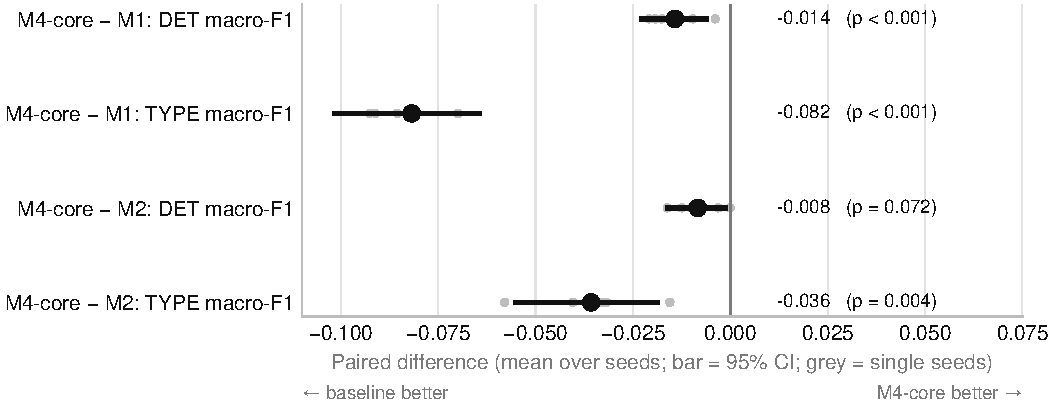
\includegraphics[width=0.9\textwidth]{figures/rq1_forest.pdf}

\vspace{2pt}
\small \textbf{H1 not supported.} Three of four differences are significant after
Holm correction, all favouring the baselines; no seed favours M4-core.
\end{frame}

\begin{frame}{RQ1: why does M4-core lose on \DET{}?}
\begin{columns}[c]
\begin{column}{0.46\textwidth}
\centering\small
\begin{tabular}{@{}lccc@{}}
\toprule
 & Recall & Precision & False alarms \\
\midrule
M2 & 0.761 & 0.722 & 345 \\
M4-core & \textbf{0.831} & 0.674 & 472 \\
\bottomrule
\end{tabular}

\vspace{4pt}
\footnotesize per seed, over 3{,}222 texts
\end{column}
\begin{column}{0.52\textwidth}
\begin{itemize}\small
\item M4-core finds \textbf{82 more} polarized texts\ldots
\item \ldots but flags \textbf{127 more} neutral ones
\item It says ``polarized'' if \emph{any} type fires
\item Its type thresholds never saw a neutral text
\item The Political threshold hit the grid floor (0.20) in 19 of 25 runs
\end{itemize}
\end{column}
\end{columns}
\vspace{8pt}
\begin{block}{}
\small The \DET{} comparison is not calibration-matched: M1 and M2 tune a
dedicated \DET{} threshold, M4-core cannot.
\end{block}
\end{frame}

\begin{frame}{The scoring scope decides the winner}
\begin{columns}[c]
\begin{column}{0.58\textwidth}
\centering
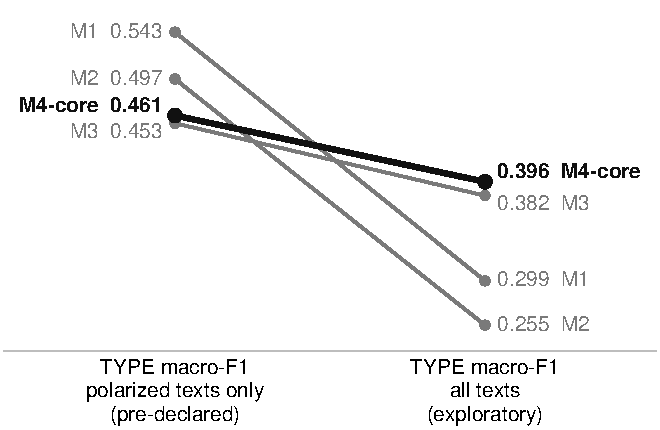
\includegraphics[width=\textwidth]{figures/scope_slope.pdf}
\end{column}
\begin{column}{0.4\textwidth}
\begin{itemize}\small
\item Pre-declared metric ignores types predicted on neutral texts
\item A consistent model can only type what it detects
\item Scored on all texts, the ranking \textbf{reverses}
\end{itemize}
\vspace{4pt}
\begin{alertblock}{Exploratory}
\footnotesize Not part of the pre-declared tests. The official scorer code is not
public, so its scope is unverified; the official data store all-zero type labels
for non-polarized texts, which is consistent with all-text scoring.
\end{alertblock}
\end{column}
\end{columns}
\end{frame}

\begin{frame}{RQ2: gating and noisy-OR tie, because two effects cancel}
\small \textbf{H2 not supported:} \TYPE{} F1 +0.008 [$-$0.009, +0.022];
macro-recall +0.006 [$-$0.014, +0.023]; Holm $p = 0.73$.

\vspace{2pt}
\centering
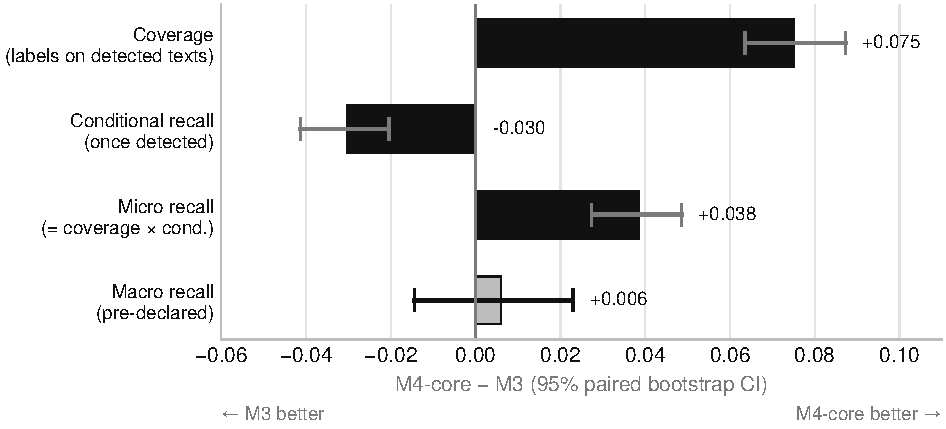
\includegraphics[width=0.84\textwidth]{figures/rq2_decomposition.pdf}

\raggedright\footnotesize
For a consistent model, label recall $=$ coverage $\times$ conditional recall.
M4-core detects more; M3 discriminates better once detected. Decomposition is exploratory.
\end{frame}

\begin{frame}{RQ2 per label: Political gains, rare labels lose}
\centering\small
\begin{tabular}{@{}lrcc@{}}
\toprule
Label & $n$ & $\Delta$ recall [95\% CI] & $\Delta$ F1 [95\% CI] \\
\midrule
Political & 1{,}150 & \textbf{+0.067} [+.055, +.078] & \textbf{+0.040} [+.033, +.048] \\
Racial/ethnic & 281 & $-$0.011 [$-$.041, +.019] & \textbf{$-$0.026} [$-$.051, $-$.003] \\
Religious & 112 & $-$0.016 [$-$.059, +.026] & $-$0.006 [$-$.041, +.030] \\
Gender/sexual & 72 & \textbf{+0.064} [+.009, +.116] & +0.039 [$-$.014, +.089] \\
Other & 126 & \textbf{$-$0.073} [$-$.113, $-$.034] & $-$0.009 [$-$.039, +.019] \\
\bottomrule
\end{tabular}

\vspace{6pt}
\raggedright
\begin{itemize}\small
\item M4-core $-$ M3; bold = interval excludes zero (exploratory)
\item The coverage gain lands on Political, which carries two thirds of all labels
\item Macro averaging weights every label equally, so gains and losses cancel
\end{itemize}
\end{frame}

\begin{frame}{RQ2: why rare labels lose, and what gating costs}
\begin{columns}[T]
\begin{column}{0.56\textwidth}
\textbf{Noisy-OR concentrates credit in Political}
\centering
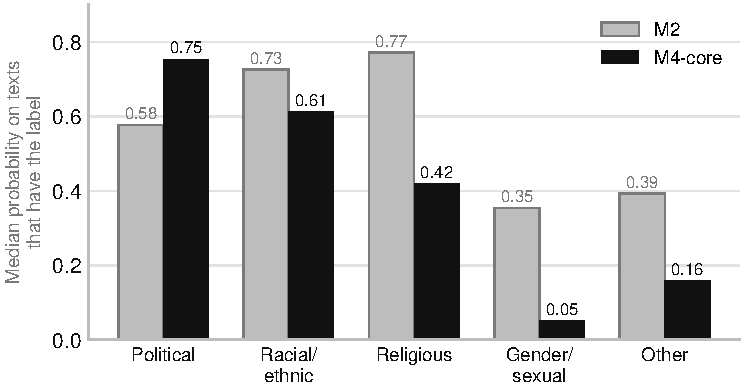
\includegraphics[width=\textwidth]{figures/probability_pairs.pdf}
\raggedright\footnotesize
Political alone can explain ``polarized'', so rare heads are pushed down
even on texts that truly have them.
\end{column}
\begin{column}{0.42\textwidth}
\textbf{Gating deletes correct labels}
\begin{itemize}\small
\item Per seed: 4{,}379 of 6{,}647 labels removed
\item 87.7\% were false alarms on neutral texts
\item But \textbf{338 correct labels} (22.9\%) were removed too
\item On 98.7\% of missed polarized texts, M2 already had a correct type
\end{itemize}
\small Error propagation from the parent decision.
\end{column}
\end{columns}
\end{frame}

\begin{frame}{Takeaways}
\begin{enumerate}
\item \textbf{Consistency has a built-in cost.}\\
  A consistent model cannot type a text it fails to detect. Where the
  constraint is enforced changes who pays, not whether.
\item \textbf{The metric decides the winner.}\\
  Scoring \TYPE{} on polarized texts vs.\ all texts reverses the ranking.
\item \textbf{Calibration is part of the model.}\\
  M4-core's main weaknesses come from its thresholds and the direction of
  the hierarchy, both testable.
\end{enumerate}
\vspace{6pt}
\small Verdicts stay frozen: RQ1 not supported, RQ2 inconclusive.
\end{frame}

\begin{frame}{Limitations}
\begin{itemize}
\item \textbf{\DET{} is not calibration-matched.} M1 and M2 tune a \DET{} threshold;
  M4-core cannot, and M1-\DET{} also selects its checkpoint on \DET{}.
\item \textbf{M1 uses twice the parameters} (368M vs.\ 184M).
\item \textbf{Some analyses were designed after seeing the results}: all-text
  scoring, the coverage decomposition, the probability profile and per-label
  differences are exploratory and uncorrected.
\item \textbf{No comparison with large models yet.} Our scores are
  cross-validation on the training set; published 12B--27B scores are on the
  official test set. RQ4 will score the official test set (labels public,
  identical to our copy) and is a secondary lens, not a headline result.
\item English only, five seeds, one GPU; official scorer scope unverified.
\end{itemize}
\end{frame}

% =====================================================================
\section{Plan}

\begin{frame}{Remaining work, in order}
\small
\begin{enumerate}
\item \textbf{Decoder extension (first).} Tune thresholds on \emph{all}
  inner-validation texts (grid 0.05--0.80); rerun M4-core and M2; compare M3 and
  M4-core at the same detection operating point.\\
  \emph{Why:} the cheapest test of whether RQ1/RQ2 are decoding artefacts.
\item \textbf{RQ5 (new): parent-to-child model M5.}\\
  \emph{Why:} a confident type should not be able to switch detection on.
\item \textbf{RQ3 (proposal): label-aware heads} and a separate Other head, on
  the variant kept after RQ5.\\
  \emph{Why:} rare labels and Other are weakest (F1 below 0.30).
\item \textbf{RQ4 (proposal, secondary lens): 184M vs.\ 12B--27B.}
  A 65--150$\times$ smaller encoder is not expected to match them; we measure
  the share of the baseline-to-best gap it closes, on the official test set.\\
  \emph{Why:} context against much larger systems, without overclaiming.
\end{enumerate}
\end{frame}

\begin{frame}{RQ5 hypothesis: reverse the direction of the hierarchy}
\centering
\resizebox{0.95\textwidth}{!}{%
\begin{tikzpicture}[
  font=\footnotesize, node distance=3mm and 3mm,
  box/.style={draw, rounded corners=1.5pt, minimum height=5mm, inner sep=2.5pt, align=center},
  enc/.style={box, fill=gray!15},
  arr/.style={-{Stealth[length=1.8mm]}, thin}
]
% M4-core
\node[font=\small\bfseries] at (2.6,1.6) {M4-core: types $\rightarrow$ detection};
\node[enc] (a1) at (0,0) {Encoder};
\node[box, right=of a1] (a2) {\TYPE{} head\\$p_k$};
\node[box, right=of a2, line width=1pt] (a3) {noisy-OR\\$1-\prod_k(1-p_k)$};
\node[right=2mm of a3] (a4) {$p_{\text{det}}$};
\draw[arr] (a1)--(a2); \draw[arr] (a2)--(a3); \draw[arr] (a3)--(a4);
% M5
\node[font=\small\bfseries] at (10.9,1.6) {M5: detection $\rightarrow$ types};
\node[enc] (b1) at (8.2,0) {Encoder};
\node[box, right=of b1, yshift=6mm] (b2) {\DET{} head\\$d$};
\node[box, right=of b1, yshift=-6mm] (b3) {conditional type head\\$q_k = P(t_k \mid d{=}1, x)$};
\node[box, anchor=west, line width=1pt] (b4) at ($(b3.east)+(9mm,6mm)$) {$p_k = d \cdot q_k$};
\draw[arr] (b1.east)--(b2.west); \draw[arr] (b1.east)--(b3.west);
\draw[arr] (b2)--(b4); \draw[arr] (b3)--(b4);
\end{tikzpicture}}

\vspace{6pt}
\raggedright\small
\begin{itemize}
\item In M5, low detection confidence softly lowers every type, and a confident
  type can no longer switch detection on; soft and hard decoders.
\item \textbf{H5a:} M5 beats M2 and the decoder-extension M4-core on \TYPE{} macro-F1.
\item \textbf{H5b (non-inferiority):} \DET{} macro-F1 within $\delta = 0.01$ of M2,
  decided by the \emph{lower end} of the 95\% interval.
\end{itemize}
\footnotesize A hypothesis to test after the decoder extension, not a result.
\end{frame}

\begin{frame}{Timeline to the final submission (Oct 31)}
\centering
\begin{tabular}{@{}lp{0.68\textwidth}@{}}
\toprule
Dates & Work \\
\midrule
Oct 2--3 & Read the official scorer; record the \TYPE{} scoring scope \\
Oct 4--6 & Decoder extension: rerun M4-core and M2 (25 runs each) \\
Oct 7--16 & RQ5: parent-to-child M5, soft and hard decoders \\
Oct 17--23 & RQ3: label-aware heads on the kept variant \\
Oct 24--27 & RQ4 (secondary): gap closure on the official test set \\
Oct 28--31 & Error analysis, final report and code release \\
\bottomrule
\end{tabular}

\vspace{8pt}
\small Each 25-run condition takes about one GPU-hour: compute is not the risk.
\end{frame}

\begin{frame}{Thank you}
\centering
\Large Questions?

\vspace{16pt}
\normalsize
\begin{tabular}{@{}rl@{}}
Code & \url{https://github.com/Rakshitagg06/ANLP_Ugh} \\[4pt]
Runs & \url{https://wandb.ai/rakshitagg06-iiit-hyderabad/anlp-project} \\
\end{tabular}
\end{frame}

% =====================================================================
\appendix
\section*{Backup}

\begin{frame}{Backup: why not let the types switch detection on?}
\textbf{Q:} M2 already had a correct type on 98.7\% of the polarized texts its
detector missed. Why not set $\hat d = \mathrm{OR}(\text{types})$ instead of gating?

\vspace{8pt}
\textbf{A:} Because M2's type head fires on \textbf{every} neutral text.
\begin{itemize}
\item M2 assigns at least one type to all 2{,}047 of 2{,}047 neutral texts
\item $\hat d = \mathrm{OR}(\text{types})$ would therefore call every text polarized
\item M4-core is the \emph{trained} version of this idea, and it still raises
  127 more false alarms per seed than M2
\item That is why RQ5 reverses the direction: detection should gate the types,
  not the other way round
\end{itemize}
\end{frame}

\begin{frame}{Backup: gating audit (M2 $\rightarrow$ M3, per seed)}
\centering\small
\begin{tabular}{@{}lrr@{}}
\toprule
Quantity & Mean & Share \\
\midrule
Type labels predicted by M2 & 6{,}647 & \\
Labels removed by gating & 4{,}379 & \\
\quad wrong, on neutral texts & 3{,}839 & 87.7\% \\
\quad wrong, on polarized texts & 202 & 4.6\% \\
\quad \textbf{correct}, on polarized texts & 338 & 7.7\% \\
Polarized texts gated (M2 detection misses) & 281 & \\
\quad with $\geq$1 correct M2 type & 277 & 98.7\% \\
\bottomrule
\end{tabular}

\vspace{6pt}
\raggedright\small
Recall cost of gating vs.\ M2: $-$0.127 macro-recall; larger on single-label texts
($-$0.239) than on multi-label texts ($-$0.161).
\end{frame}

\begin{frame}{Backup: progress against the proposal}
\centering\small
\begin{tabular}{@{}ll@{}}
\toprule
Proposal item & Status \\
\midrule
Stratified 5-fold CV, metrics, LVR & Done \\
M1 and M2 (5 folds $\times$ 5 seeds) & Done \\
M3 gating & Done (re-implemented) \\
M4 noisy-OR & Done as M4-core \\
Full ladder and paired tests & Done (ahead of plan) \\
Label-aware attention, Other head & Kept as RQ3 \\
TF-IDF, BERT, RoBERTa baselines & Deferred \\
Comparison with 12B--27B systems & Kept as RQ4 (secondary) \\
\bottomrule
\end{tabular}
\end{frame}

\end{document}
